\section{Konstruktion neuer Algebren}

In diesem Kapitel werden drei verschiedene Konstruktionen vorgestellt um aus bereits gegebenen Algebren neue zu gewinnen.

\begin{definition}
    Sei $\mathfrak{A}=(A,(f^\mathfrak{A}_i)_{i\in I})$ eine Algebra und $S\subseteq A$. Dann heißt das Tupel $\mathfrak{S}=(S,(f^\mathfrak{A}_i|_{S^{n_i}})_{i\in I})$\footnote{Zwecks besserer Lesbarkeit werden wir dafür meist $\mathfrak{S}=(S,(f^\mathfrak{S}_i)_{i\in I})$ schreiben.}
    \emph{Subalgebra}\index{Subalgebra} oder \emph{Unteralgebra}\index{Unteralgebra} von $\mathfrak{A}$, wenn
    \begin{itemize}[topsep=0pt, label={--}]
        \item $\forall i\in I\forall a_1,\ldots,a_{n_i}\in S:f^\mathfrak{A}_i(a_1,\ldots,a_{n_i})\in S.$\tab ($S$ \emph{ist abgeschlossen gegenüber allen} $f_i$)
    \end{itemize}
    Wir schreiben in diesem Fall $\mathfrak{S}\le \mathfrak{A}$.
\end{definition}

\begin{example}
    Sei $\mathfrak{V}=(V,+,0,-,(m_k)_{k\in\mathfrak{K}})$ ein Vektorraum über einem Körper $\mathfrak{K}$. Dann gilt für
    jeden Untervektorraum $U$ von $V$: $\mathfrak{U}=(U,+,0,-,(m_k)_{k\in\mathfrak{K}})\le \mathfrak{V}$. 
    
    Weitere Beispiele für Unteralgebren sind $(\mathbb{N},+)\le(\mathbb{Z},+)$ und $(\Sl_n(K),\cdot)\le (\Gl_n(K),\cdot)$.
\end{example}

\begin{proposition}\label{prop:unteralgebra}
    Sei $\mathfrak{A}=(A,(f^\mathfrak{A}_i)_{i\in I})$ eine Algebra, $s\approx t$ ein Gesetz und gelte $\mathfrak{A}\models s\approx t$.
    Dann gilt für jede Unteralgebra $\mathfrak{S}$ von $\mathfrak{A}$ auch $\mathfrak{S}\models s\approx t$.
\end{proposition}

\begin{proof}
    Laut Definition gilt für alle Variablenbelegungen $\varphi:\var(s)\cup \var(t)\to A:\bar{\varphi}(s)=\bar{\varphi}(t)$.
    Wegen $S\subseteq A$ ist diese Bedingung insbesondere für alle $\varphi : \var(s) \cup \var(t) \to S$ erfüllt, also gilt $\mathfrak{S}\models s\approx t$.
\end{proof}

\begin{remark}
    Sei $\mathfrak{V}=(V,+,0,-,(m_k)_{k\in\mathfrak{K}})$ ein Vektorraum über einem Körper $\mathfrak{K}$.
    Dann ist $x\approx 0$ ein Gesetz, welches in $(\{0\},+,0,-)$ erfüllt ist, jedoch nicht in $\mathfrak{V}$.
    Wir sehen also, dass die Umkehrung von Proposition \ref{prop:unteralgebra} nicht gilt.
\end{remark}

\begin{corollary}\label{corollary:sub-varietaeten}
    Varietäten sind abgeschlossen unter der Bildung von Unteralgebren.
\end{corollary}

\begin{remark}
    Eine Folgerung ist unmittelbar, dass die Klasse der Körper keine Varietät bildet,
    denn $(\mathbb{Z},+,0,-,\cdot,1)$ ist eine Unteralgebra von $(\mathbb{Q},+,0,-,\cdot,1)$, aber die ganzen Zahlen stellen keinen Körper dar.
\end{remark}

\begin{remark}
    An dieser Stelle können wir den Unterschied der gegebenen Definitionen einer Gruppe feststellen,
    denn $(\mathbb{N},+)$ ist eine Unteralgebra von $(\mathbb{Z},+)$, jedoch keine Gruppe im Sinne von 
    \cref{rem:alternativegruppe}. Das bedeutet, dass in der Sprache $+$ die Klasse der Gruppen keine Varietät bildet.
\end{remark}

\notedate{09.03.2023}
\vspace*{-\lineskip}

\begin{proposition}
    Sei $\mathfrak{A}=(A,(f^\mathfrak{A}_i)_{i\in I})$ eine Algebra und $(\mathfrak{S}_j = (S_j, (f_i^{\mathfrak{S}_j})_{i \in I}))_{j\in J}$ eine Familie von Unteralgebren
    von $\mathfrak{A}$. Dann ist auch $\mathfrak{S} = \bigcap_{j \in J} \mathfrak{S}_j := (\bigcap_{j\in J}S_j,(f^\mathfrak{A}_i\vert_{\bigcap_{j\in J}S_j})_{i\in I})$ eine Unteralgebra von $\mathfrak{A}$.
\end{proposition}

\begin{proof}
    Für $S:=\bigcap_{j\in J}S_j$ gilt offensichtlich $S\subseteq A$, also bleibt lediglich die Abgeschlossenheit bezüglich
    der Funktionen $f^\mathfrak{S}_i$ zu zeigen. Seien $a_1,\ldots,a_{n_i}\in S$ beliebig. Dann gilt für alle
    $j\in J:a_1,\ldots,a_{n_i}\in S_j$ und da $\mathfrak{S}_j$ eine Unteralgebra von $\mathfrak{A}$ ist auch $f^{\mathfrak{S}_j}_i(a_1,\ldots,a_{n_i})\in S_j$.
    Das ist genau die Definition von $f^\mathfrak{S}(a_1,\ldots,a_{n_i})\in \bigcap_{j\in J}S_j=S$, also ist $\mathfrak{S}=(S,(f^\mathfrak{S}_i)_{i\in I})$ eine Unteralgebra von $\mathfrak{A}$.
\end{proof}

\begin{corollary}
    Sei $\mathfrak{A}=(A,(f^\mathfrak{A}_i)_{i\in I})$ eine Algebra und $S\subseteq A$. Dann ist die von $S$ \emph{erzeugte Unteralgebra}\index{erzeugte Unteralgebra}\index{Unteralgebra!erzeugte} von 
    $\mathfrak{A}$ definiert durch $\langle S\rangle:=\bigcap\{\mathfrak{U} \mid S\subseteq U\land \mathfrak{U} = (U,(f^\mathfrak{A}_i)_{i\in I})\le \mathfrak{A}\}$
    die kleinste $S$ enthaltende Unteralgebra von $\mathfrak{A}$.
\end{corollary}

\begin{definition}
    Sei $\mathfrak{A}=(A,(f^\mathfrak{A}_i)_{i\in I})$ eine Algebra und $S\subseteq A$. Die Menge $S_\infty$ ist rekursiv
    definiert durch
    \[S_0:=S, \quad S_{k+1}:=S_k\cup\{f^\mathfrak{A}_i(a_1,\ldots,a_{n_i} \mid i\in I\land a_1,\ldots a_{n_i}\in S_k)\},\quad S_\infty:=\bigcup_{k\geq 0}S_k.\]
\end{definition}

\begin{example}
    Diese Skizze zeigt die anschauliche Motiviation der vorhergehenden Definition.

    \begin{figure}[H]
        \centering
        \resizebox{6cm}{6cm}{
        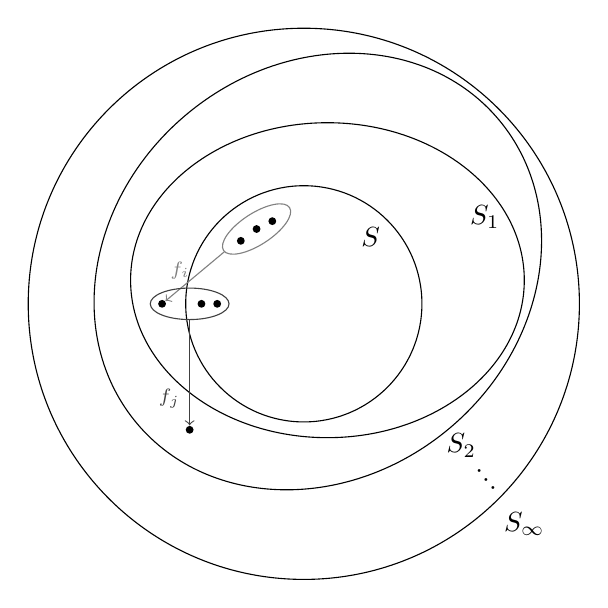
\begin{tikzpicture}
            \draw (0,0) circle (1.5);
            \node at (0.85, 0.85) {$S$};
            
            \draw (0.3,0.3) ellipse (2.5 and 2); 
            \node at (2.3, 1.1) {$S_1$};
            
            \draw[rotate=40] (0.4,0.2) ellipse (3 and 2.6); 
            \node at (2, -1.8) {$S_2$};
            
            \draw (0,0) circle (3.5);
            \node at (2.8, -2.8) {$S_\infty$};
            \node[rotate=38] at (2.25,-2.15) {$\vdots$};

            \node[circle,fill,inner sep=1pt] (p1) at (-0.8, 0.8){};
            \node[circle,fill,inner sep=1pt] (p2) at (-0.6, 0.95){};
            \node[circle,fill,inner sep=1pt] (p3) at (-0.4, 1.05){};
            \draw[gray, rotate=33] (p2) ellipse (0.5 and 0.2);

            \node[circle,fill,inner sep=1pt] (p4) at (-1.8, 0){};

            \draw[->, gray] (-1.01, 0.66) -- node[above, near end] {\scriptsize $f_i$} (p4);

            \node[circle,fill,inner sep=1pt] (p5) at (-1.3, 0){};
            \node[circle,fill,inner sep=1pt] (p6) at (-1.1, 0){};

            \draw[darkgray] (-1.45,0) ellipse (0.5 and 0.2);

            \node[circle,fill,inner sep=1pt] (p7) at (-1.45, -1.6){};

            \draw[->, darkgray] (-1.45, -0.2) -- node[left, near end] {\scriptsize $f_j$} (p7);

        \end{tikzpicture}
        }
        \caption{Subalgebra von unten}
    \end{figure}
\end{example}

\begin{proposition}
    Sei $\mathfrak{A}=(A,(f^\mathfrak{A}_i)_{i\in I})$ eine Algebra, $S\subseteq A$ und $X$ eine beliebige Menge. Dann gelten die beiden Identitäten:
    \begin{enumerate}
        \item $\langle S\rangle=S_\infty$
        \item $\langle S\rangle=\{t^\mathfrak{A}(a_1,\ldots,a_n) \mid a_1,\ldots,a_n\in S, t \in T(X) \}$
    \end{enumerate}
\end{proposition}
\begin{proof} In beiden Behauptungen wird die gegenseitige Inklusion von zwei Mengen gezeigt.
    \begin{enumerate}
        \item Da $S_\infty$\footnote{Hier wird die Algebra für bessere Lesbarkeit mit der Trägermenge identifiziert} eine $S$ enthaltende Unteralgebra von $A$ ist, folgt aus der Definition der
        erzeugten Unteralgebra, dass $\langle S\rangle\subseteq S_\infty$ gilt.
        Für die andere Inklusion wird mittels Induktion gezeigt, dass für alle $k\in\mathbb{N}:S_k\subseteq \langle S\rangle$ gilt,
        woraus schließlich auch $S_\infty=\bigcup_{k\in\mathbb{N}}S_k\subseteq \langle S\rangle$ folgt.

        Induktionsanfang $(k=0)$: Per Definitionem der erzeugten Algebra gilt $S_0=S\subseteq \langle S\rangle$. \\
        Induktionsschritt $(k\to k+1)$: Sei nun $a\in S_{k+1}$ beliebig. Falls $a\in S_k$ ist, so folgt aus
        der Induktionsvoraussetzung dass $a\in \langle S\rangle$ gilt. Andernfalls existieren ein $i\in I$ und
        $a_1,\ldots,a_{n_i}\in S_{k}$, sodass $a=f_i^{\mathfrak{A}}(a_1,\ldots,a_{n_i})$. Auch hier kann die Induktionsvoraussetzung
        angewandt werden, weshalb $a_1,\ldots,a_{n_i}\in \langle S\rangle$ ist. Da $(\langle S\rangle,(f_i^{\mathfrak{A}})_{i\in I})$ eine Unteralgebra
        von $\mathfrak{A}$ ist, gilt auch $a=f_i^{\mathfrak{A}}(a_1\ldots,a_{n_i})\in\langle S\rangle$. Daraus folgt die gewünschte Mengeninklusion
        $S_{k+1}\subseteq \langle S\rangle$.

        \item Definiere $M:=\{t^\mathfrak{A}(a_1,\ldots,a_n)\vert a_1,\ldots,a_n\in S\land t\in T(X)\}$.
        Es gilt $S\subseteq M$, da die Projektionen $\pi_j^{(n)}:A^n\to A, (a_1,\ldots,a_n)\mapsto a_j$ Termfunktionen sind.
        Außerdem kann gezeigt werden, dass $(M,(f_i)_{i\in I})$ eine Unteralgebra von $\mathfrak{A}$ ist. Sei $i\in I$ beliebig
        und seien $b_1,\ldots,b_{n_i}\in M$, dann können diese Elemente als $b_j=t_j^\mathfrak{A}(a_1^{(j)},\ldots,a_{m_j}^{(j)})$
        mit $a_1^{(j)},\ldots,a_{m_j}^{(j)}\in S$ für $j\in \{1,\ldots,n_i\}$ dargestellt werden. Definiert man nun $a:=f^\mathfrak{A}_i(b_1,\ldots,b_{n_i})$
        und den Term $t:=f_i^\mathfrak{T}(t_1(x_1^{(1)},\ldots,x_{m_1}^{(1)}),\ldots,t_{n_i}(x_1^{(n_i)},\ldots,x_{m_{n_i}}^{(n_i)}))$,
        so erhält man eine passende Termfunktion, das heißt es gilt $t^\mathfrak{A}(a_1^{(1)},\ldots,a_{m_1}^{(1)},\ldots,a_1^{(n_i)},\ldots,a_{m_{n_i}}^{(n_i)})=a$,
        also insbesondere $a\in M$. Für die andere Mengeninklusion ist erneut eine Induktion nötig.
        Sei $a=t^\mathfrak{A}(a_1,\ldots,a_n)\in M$ beliebig. Zu zeigen ist, dass $a\in \langle S\rangle$ gilt,
        wobei dies mittels Induktion nach der Stufe von $t$ gezeigt wird.

        Induktionsanfang $(k=0)$: Dann ist der Term $t$ eine Variable $x_j$ und die Termfunktion
        $t^\mathfrak{A}$ ist eine Projektion $a=t^\mathfrak{A}(a_1,\ldots,a_n)=\pi_j^n(a_1,\ldots,a_n)=a_j\in S\subseteq \langle S\rangle$.\\
        Induktionsschritt $(m<k\to k)$: Dann ist $t=f^\mathfrak{T}_i(t_1,\ldots,t_{n_i})$ und
        $a=t^\mathfrak{A}(a_1,\ldots,a_{n_i})=f^\mathfrak{A}_i(t^\mathfrak{A}_1(a_1,\ldots,a_n),\ldots,t^\mathfrak{A}_{n_i}(a_1,\ldots,a_n))\in\langle S\rangle$,
        da die Terme $t^\mathfrak{A}_j$ für $j\in\{1,\ldots,n_i\}$ kleinere Stufe als $k$ haben. Daher
        sind die Argumente nach Induktionsvoraussetzung in $\langle S\rangle$ und damit auch
        der Funktionswert.
    \end{enumerate}
\end{proof}

\begin{corollary}
    Sei $\mathfrak{A}=(A,(f^\mathfrak{A}_i)_{i\in I})$ eine Algebra, $S=\{s_1,\ldots,s_n\}\subseteq A$ und $X$ eine beliebige Menge.
    Dann gilt für die von $S$ erzeugte Unteralgebra
    $$ \langle S\rangle=\{t^\mathfrak{A}(s_1,\ldots,s_n)\mid t(x_1,\ldots,x_n)\in T(X)\}. $$
\end{corollary}

\begin{proof}
    Es gilt klarerweise $\langle S\rangle\supseteq \{t^\mathfrak{A}(s_1,\ldots,s_n)\mid t(x_1,\ldots,x_n)\in T(X)\}$.
    Sei $a\in\langle S\rangle$ beliebig. Dann existiert ein Term $t$ und es existieren $a_1,\ldots,a_\ell\in S$,
    sodass $a=t^\mathfrak{A}(a_1,\ldots,a_\ell)$. Mit dem Term $\tilde{t}(x_1,\ldots,x_n):=t(y_1,\ldots,y_\ell)$, wobei $y_i:=x_j\leftrightarrow a_i=s_j$
    erhält man $\tilde{t}^\mathfrak{A}(s_1,\ldots,s_n)=t^\mathfrak{A}(a_1,\ldots,a_\ell)=a\in\{t^\mathfrak{A}(s_1,\ldots,s_n)\mid t(x_1,\ldots,x_n)\in T(X)\}.$
\end{proof}

\begin{remark}
    Für eine beliebige Algebra ist mit $\Sub(\mathfrak{A}):=\{\mathfrak{U}\mid \mathfrak{U}\le \mathfrak{A}\}$ durch
    $(\Sub(\mathfrak{A}),\subseteq)$ eine Halbordnung gegeben. Weiter ist $(\Sub(\mathfrak{A},\land,\lor))$,
    wobei $U_1\land U_2:=U_1\cap U_2$ und $U_1\lor U_2:=\langle U_1\cup U_2\rangle$, ein Verband.
\end{remark}

\begin{remark}
    Das kartesische Produkt von Mengen $(M_i)_{i \in I}$ ist definiert als 
    $$ \prod_{i \in I} M_i := \left\{f: I \to \bigcup_{i \in I} M_i \mid \forall i \in I: f(i) \in M_i \right\}. $$

    Genau genommen sind die Elemente von Produktmengen also Funktionen. Im Folgenden werden statt Funktionsnotation oft Familien (welche nur eine andere Notation für Funktionen sind) und bei endlicher Indexmenge $I$ auch Tupel geschrieben.
    
\end{remark}

\begin{definition}
    Sei $\tau = (n_i)_{i\in I}$ ein Typ und sei $(\mathfrak{A}_j)_{j\in J}$ eine Familie von Algebren dieses Typs.
    Dann heißt $\mathfrak{A}:=\prod_{j\in J}\mathfrak{A}_j=(\prod_{j\in J}A_j,(f^\mathfrak{A}_i)_{i\in I})$ \emph{Produktalgebra}\index{Produktalgebra},
    wobei die Operationen durch $f^\mathfrak{A}_i: \mathfrak{A}^{n_i} \to \mathfrak{A}, ((a_j^{(1)})_{j \in J}, \ldots (a_j^{(n_i)})_{j \in J}) \mapsto (f^{\mathfrak{A}_j}_i(a_j^{(1)}, \ldots, a_j^{(n_i)}))_{j \in J}$
    definiert werden.
\end{definition}

\begin{example}
    \Cref{fig:produktalgebra} visualisiert die Bildung einer Produktalgebra.
\end{example}

\begin{figure}[H]
    \centering
    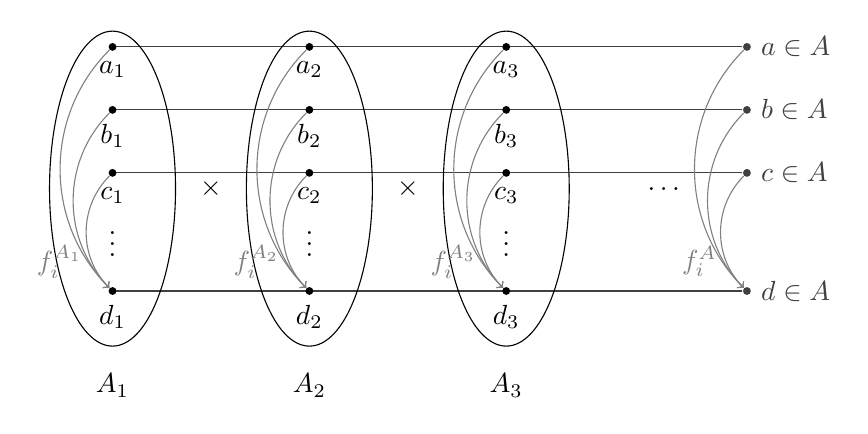
\begin{tikzpicture}
        
        \draw[darkgray] (0, 1.8) -- (8, 1.8) node[right, circle,fill, inner sep=1pt, label=right:$a \in \mathfrak{A}$] (a) {};
        \draw[darkgray] (0, 1) -- (8, 1) node[right, circle,fill, inner sep=1pt, label=right:$b \in \mathfrak{A}$] (b) {};
        \draw[darkgray] (0, 0.2) -- (8, 0.2) node[right, circle,fill, inner sep=1pt, label=right:$c \in \mathfrak{A}$] (c) {};
        \draw[darkgray] (0, -1.3) -- (8, -1.3) node[right, circle,fill, inner sep=1pt, label=right:$d \in \mathfrak{A}$] (d) {};

        \draw (0,0) ellipse (0.8 and 2);
        \node[circle,fill,inner sep=1pt,label=below:$a_1$] (a1) at (0, 1.8){};
        \node[circle,fill,inner sep=1pt,label=below:$b_1$] (b1) at (0, 1){};
        \node[circle,fill,inner sep=1pt,label=below:$c_1$] (c1) at (0, 0.2){};
        \node at (0, -0.6) {$\vdots$};
        \node[circle,fill,inner sep=1pt,label=below:$d_1$] (d1) at (0, -1.3){};
        \node at (0, -2.5) {$\mathfrak{A}_1$};

        \node at (1.25, 0) {$\times$};

        \draw (2.5,0) ellipse (0.8 and 2);
        \node[circle,fill,inner sep=1pt,label=below:$a_2$] (a2) at (2.5, 1.8){};
        \node[circle,fill,inner sep=1pt,label=below:$b_2$] (b2) at (2.5, 1){};
        \node[circle,fill,inner sep=1pt,label=below:$c_2$] (c2) at (2.5, 0.2){};
        \node at (2.5, -0.6) {$\vdots$};
        \node[circle,fill,inner sep=1pt,label=below:$d_2$] (d2) at (2.5, -1.3){};
        \node at (2.5, -2.5) {$\mathfrak{A}_2$};

        \node at (3.75, 0) {$\times$};

        \draw (5,0) ellipse (0.8 and 2);
        \node[circle,fill,inner sep=1pt,label=below:$a_3$] (a3) at (5, 1.8){};
        \node[circle,fill,inner sep=1pt,label=below:$b_3$] (b3) at (5, 1){};
        \node[circle,fill,inner sep=1pt,label=below:$c_3$] (c3) at (5, 0.2){};
        \node at (5, -0.6) {$\vdots$};
        \node[circle,fill,inner sep=1pt,label=below:$d_3$] (d3) at (5, -1.3){};
        \node at (5, -2.5) {$\mathfrak{A}_3$};

        \node at (7,0) {$\ldots$};

        \draw[->, gray] (a1) edge [bend right=45] (d1);
        \draw[->, gray] (b1) edge [bend right=45] (d1);
        \draw[->, gray] (c1) edge [bend right=45] node[left, near end] {$f_i^{\mathfrak{A}_1}$} (d1);

        \draw[->, gray] (a2) edge [bend right=45] (d2);
        \draw[->, gray] (b2) edge [bend right=45] (d2);
        \draw[->, gray] (c2) edge [bend right=45] node[left, near end] {$f_i^{\mathfrak{A}_2}$} (d2);

        \draw[->, gray] (a3) edge [bend right=45] (d3);
        \draw[->, gray] (b3) edge [bend right=45] (d3);
        \draw[->, gray] (c3) edge [bend right=45] node[left, near end] {$f_i^{\mathfrak{A}_3}$} (d3);

        \draw[->, gray] (a) edge [bend right=45] (d);
        \draw[->, gray] (b) edge [bend right=45] (d);
        \draw[->, gray] (c) edge [bend right=45] node[left, near end] {$f_i^{\mathfrak{A}}$} (d);
    \end{tikzpicture}
    \caption{Visualisierung von Produktalgebren}
    \label{fig:produktalgebra}
\end{figure}

\begin{remark}
    Ist $\mathfrak{A}=\prod_{j\in J}\mathfrak{A}_j$ eine Produktalgebra und $j\in J$, so ist durch die Projektionsabbildung
    $\pi_j:\mathfrak{A}\to \mathfrak{A}_j, (a_j)_{j \in J}\mapsto a_j$ ein surjektiver Homomorphismus gegeben.
\end{remark}

\begin{proposition}
    Seien $(f_i)_{i\in I}$ eine Signatur, $s\approx t$ ein Gesetz in dieser Sprache, $(\mathfrak{A}_j)_{j\in J}$
    eine Familie von Algebren in der Signatur und es gelte für alle $j\in J:\mathfrak{A}_j\models s\approx t$.
    Dann gilt auch $\mathfrak{A}:=\prod_{j\in J}\mathfrak{A}_j\models s\approx t$.
\end{proposition}

\begin{proof}
    Es ist hinreichend zu zeigen, dass $s^\mathfrak{A}=t^\mathfrak{A}$ gilt. Seien $\vec a^{(1)} = (a_j^{(1)})_{j \in J}, \ldots,\vec a^{(n)}\in A$ beliebig.
    Dann gilt laut Voraussetzung für alle $j\in J:s^{\mathfrak{A}_j}(a^{(1)}_j,\ldots,a^{(n)}_j)) = t^{\mathfrak{A}_j}(a^{(1)}_j,\ldots,a^{(n)}_j))$.
    Daher folgt $s^\mathfrak{A}(\vec a^{(1)},\ldots,\vec a^{(n)})_j=s^{\mathfrak{A}_j}(a^{(1)}_j,\ldots,a^{(n)}_j)) = t^{\mathfrak{A}_j}(a^{(1)}_j,\ldots,a^{(n)}_j))=t^\mathfrak{A}(\vec a^{(1)},\ldots,\vec a^{(n)})_j$
    für alle $j\in J$, also insbesondere $s^\mathfrak{A}(\vec a^{(1)},\ldots,\vec a^{(n)})=t^\mathfrak{A}(\vec a^{(1)},\ldots,\vec a^{(n)})$ und damit $s^\mathfrak{A}=t^\mathfrak{A}.$
\end{proof}

\begin{corollary}\label{corollary:prod-varietaeten}
    Varietäten sind abgeschlossen unter der Bildung von Produkten.
\end{corollary}

\begin{remark}
    Auch an dieser Stelle wird deutlich, dass die Klasse der Körper keine Varietät ist. Für einen Körper $\mathfrak{K}$
    und den Produktraum $\mathfrak{K}\times \mathfrak{K}$ gilt $(1,0)\cdot (0,1)=(0,0)$. Da Körper immer nullteilerfrei sind,
    kann dieser Produktraum folglich kein Körper sein.
\end{remark}

\notedate{15.03.2023}

\begin{definition}
    Sei $\mathfrak{A}=(A,(f^\mathfrak{A}_i)_{i\in I})$ eine Algebra, $m\in\mathbb{N}$ und $R\subseteq A^m$ eine $m$-stellige
    Relation auf $A$. Dann heißt $R$ \emph{invariant unter $\mathfrak{A}$}\index{invariante Relation}\index{Relation!invariant}, wenn
    \begin{itemize}[topsep=0pt, label={--}]
        \item $\forall i\in I:\forall r^{(1)},\ldots,r^{(n_i)}\in R:(f_i(r_1^{(1)},\ldots,r_1^{(n_i)}),\ldots,f_i(r_m^{(1)},\ldots,r_m^{(n_i)}))\in R$.
    \end{itemize}
\end{definition}

\begin{definition}
    Sei $\mathfrak{A}=(A,(f^\mathfrak{A}_i)_{i\in I})$ eine Algebra und $\sim\;\subseteq A^2$ eine Äquivalenzrelation.
    Wenn $\sim$ invariant unter $\mathfrak{A}$ ist, dann heißt $\sim$ \emph{Kongruenzrelation}\index{Kongruenzrelation}. Außerdem wird damit die Menge
    Con$(\mathfrak{A}):=\{\sim\subseteq A^2\mid \;\sim \text{ ist Kongruenzrelation auf }\mathfrak{A}\}$ definiert.
\end{definition}

\begin{example}
    Sei $X$ eine Menge, $(f_i)_{i\in I}$ eine Signatur und $\mathfrak{T}=(T,(f^\mathfrak{T}_i)_{i\in I})$ die Termalgebra über $X$.
    Sei außerdem $\mathfrak{A}=(A,(f^\mathfrak{A}_i)_{i\in I})$ eine Algebra in derselben Signatur. Dann ist durch
    $t\sim s:\leftrightarrow t^\mathfrak{A}=s^\mathfrak{A}$ auf $\mathfrak{T}$ eine Kongruenzrelation gegeben.
\end{example}

\begin{example}
    Für jede beliebige Algebra $\mathfrak{A}=(A,(f^\mathfrak{A}_i)_{i\in I})$ sind durch die beiden Relationen $\sim_1=A^2$ und $\sim_2=\{(a,a)\mid a\in A\}$
    Kongruenzrelationen auf $\mathfrak{A}$ gegeben. Diese nennt man daher auch \emph{triviale Kongruenzrelationen}\index{Kongruenzrelation!trivial}.
\end{example}

\begin{remark}
    Für eine beliebige Algebra $\mathfrak{A}$ ist durch $(\text{Con}(A),\subseteq)$ eine Halbordnung gegeben.
    Da es zu zwei Kongruenzrelationen bezüglich der Mengeninklusion immer ein Supremum und Infimum gibt,
    entsteht sogar ein Verband.
\end{remark}

\begin{definition} \label{def:einfache-algebra}
    Eine Algebra $\mathfrak{A}$ heißt \emph{einfach}\index{Algebra!einfache}, wenn es keine nicht-trivialen Kongruenzrelationen gibt.
\end{definition}

\begin{definition}
    Sei $\mathfrak{A}=(A,(f^\mathfrak{A}_i)_{i\in I})$ eine Algebra und sei $\sim\subseteq A^2$ eine Kongruenzrelation.
    Dann heißt $\mathfrak{A}/_\sim:=(A/_\sim,(f^{\mathfrak{A}/_\sim}_i)_{i\in I})$ \emph{Faktoralgebra}\index{Faktoralgebra} von $\mathfrak{A}$,
    wobei $A/_\sim=\{[a]_\sim\mid a\in A\}$ die Menge der Äquivalenzklassen\footnote{Für die Äquivalenzklassen einer Äquivalenzrelation
    wird häufig $[a]$ statt $[a]_\sim$ geschrieben.} ist und die Funktionen definiert\footnote{Dass diese Funktionen tatsächlich wohldefiniert sind,
    folgt direkt aus der Definition der Invaranz einer Kongruenzrelation unter der Algebra.} sind durch
    $f^{\mathfrak{A}/_\sim}([a_1]_\sim,\ldots,[a_{n_i}]_\sim):=[f_i(a_1,\ldots,a_{n_i})]_\sim.$
\end{definition}

\begin{example}
    Betrachten wir die Algebra $(\mathbb{Z},+,\cdot)$ und definieren darauf die Kongruenzrelation
    $a\sim b:\leftrightarrow \exists k\in\mathbb{Z}(a-b=k\cdot m)$, so stellt $(\mathbb{Z}_m,+,\cdot)=(\mathbb{Z},+,\cdot)/_\sim$
    eine Faktoralgebra dar. Man bemerke außerdem, dass in $(\mathbb{Z}_m,+,\cdot)$ beispielsweise das Gesetz
    $\forall x(\overbrace{x +\ldots + x}^{m+1\;\text{mal}}=x)$ gilt, während dieses in $(\mathbb{Z},+,\cdot)$ nicht gilt. Es können also in einer Faktoralgebra mehr Gesetze erfüllt sein, als in der ursprünglichen Algebra.
\end{example}

\begin{remark}
    Sei $\mathfrak{A}$ eine beliebige Algebra und $\sim$ eine Kongruenzrelation. Dann ist die \emph{kanonische Faktorabbildung}\index{kanonische Faktorabbildung} oder \emph{kanonische Projektion}\index{kanonische Projektion}
    $\varphi:A\to A/_\sim, a\mapsto [a]_\sim$ ein surjektiver Homomorphismus, das heißt
    Faktoralgebren sind homomorphe Bilder von Algebren. Der folgende Satz liefert in einem gewissen Sinn die Umkehrung.
\end{remark}

\begin{lemma}
    Seien $\mathfrak{A}=(A,(f^\mathfrak{A}_i)_{i\in I})$ und $\mathfrak{B}=(B,(f^\mathfrak{B}_i)_{i\in I})$ Algebren vom selben Typ
    und sei $h:\mathfrak{A}\to \mathfrak{B}$ ein Homomorphismus. Dann ist $\ker h:=\{(a,b)\in A^2\mid h(a)=h(b)\}$ eine Kongruenzrelation auf $\mathfrak{A}$.
\end{lemma}

\begin{proof}
    Es sei $i\in I$ beliebig und $a_1\ldots,a_{n_i},b_1\ldots,b_{n_i}\in A$ mit $(a_j,b_j)\in \ker h$ für alle $j\in \{1,\ldots,n_i\}$.
    Laut Definition gilt also $h(a_j)=h(b_j)$ für alle $j\in\{1,\ldots,n_i\}$ und daher auch
    $h(f^\mathfrak{A}_i(a_1,\ldots,a_{n_i}))=f^\mathfrak{B}_i(h(a_1),\ldots,h(a_{n_i}))=f^\mathfrak{B}_i(h(b_1),\ldots,h(b_{n_i}))=h(f^\mathfrak{A}_i(b_1,\ldots,b_{n_i}))$,
    also ist $(f^\mathfrak{A}_i(a_1,\ldots,a_{n_i}),f^\mathfrak{A}_i(b_1,\ldots,b_{n_i}))\in\ker h$. Damit ist $\ker h$ invariant unter $\mathfrak{A}$
    und da es sich offensichtlich um eine Äquivalenzrelation handelt, ist $\ker h$ eine Kongruenzrelation auf $\mathfrak{A}$.
\end{proof}

\begin{theorem}[Homomorphiesatz]\index{Homomorphiesatz}
    Seien $\mathfrak{A}=(A,(f^\mathfrak{A}_i)_{i\in I})$ und $\mathfrak{B}=(B,(f^\mathfrak{B}_i)_{i\in I})$ zwei Algebren
    in derselben Signatur, $\varphi:\mathfrak{A}\to \mathfrak{A}/_{\ker h}$ die kanonische Faktorabbildung und sei $h:\mathfrak{A}\to \mathfrak{B}$ ein Homomorphismus.
    Dann existiert genau ein Homomorphismus $\tilde{h}:\mathfrak{A}/_{\ker h}\to \mathfrak{B}$ mit $h=\tilde{h}\circ \varphi$. Dieser Homomorphismus
    ist injektiv und, falls $h$ surjektiv ist, auch surjektiv.
    \begin{figure}[H]
        \centering
        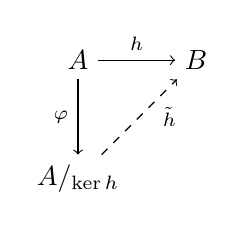
\begin{tikzpicture}
            \node (a) at (0,0) {$\mathfrak{A}$};
            \node (a_fak) at (0,-1.5) {$\mathfrak{A}/_{\ker h}$};
            \node (b) at (1.5,0) {$\mathfrak{B}$};

            \draw[->] (a) -- node[left] {\scriptsize $\varphi$} (a_fak);
            \draw[->] (a) -- node[above] {\scriptsize $h$} (b);
            \draw[dashed,->] (a_fak) -- node[right=5pt] {\scriptsize $\tilde{h}$} (b);
        \end{tikzpicture}
        \caption{Visualisierung der Aussage des Homomorphiesatzes}
    \end{figure}
\end{theorem}

\begin{proof}
    Für die Surjektivität von $\tilde{h}$ ist nichts zu zeigen. Der übrige Beweis ist in vier Schritte gegliedert.

    Eindeutigkeit: Seien $\tilde{h}$ und $\hat{h}$ zwei Homomorphismen von $\mathfrak{A}/_{\ker h}$ nach $\mathfrak{B}$ mit den geforderten Eigenschaften.
    Dann gilt für $a\in A$ beliebig $\hat{h}([a])=h(a)=\tilde{h}([a])$, also $\hat{h}=\tilde{h}$.

    Existenz: Sei $[a]\in A/_{\ker h}$ beliebig und definiere $\tilde{h}([a]):=h(a)$. Diese Abbildung ist wohldefiniert,
    da aus $[a]=[b]$ laut Definition $h(a)=h(b)$ folgt, das heißt die Definition ist unabhängig von der Wahl des Repräsentanten.

    Homomorphismus: Sei $i\in I$ und seien $[a_1],\ldots,[a_{n_i}]\in A/_{\ker h}$ beliebig. Dann gilt laut Definition
    $\tilde{h}(f^{\mathfrak{A}/_{\ker h}}_i([a_1],\ldots,[a_{n_i}]))=\tilde{h}([f^\mathfrak{A}_i(a_1,\ldots,a_{n_i})])=h(f^\mathfrak{A}_i(a_1,\ldots,a_{n_i}))=f^\mathfrak{B}_i(h(a_1),\ldots,h(a_{n_i}))=f^\mathfrak{B}_i(\tilde{h}([a_1]),\ldots,\tilde{h}([a_{n_i}]))$,
    also ist $\tilde{h}$ ein Homomorphismus.

    Injektivität: Seien $[a],[b]\in A/_{\ker h}$ beliebig mit $\tilde{h}([a])=\tilde{h}([b])$. Dann folgt laut Definition
    $h(a)=h(b)$, also $(a,b)\in\ker h$ und damit $[a]=[b]$.
\end{proof}

\begin{proposition}
    Seien $\mathfrak{A}=(A,(f^\mathfrak{A}_i)_{i\in I})$ eine Algebra, $s\approx t$ ein Gesetz und gelte $\mathfrak{A}\models s\approx t$.
    Dann gilt für jede Faktoralgebra $\mathfrak{A}/_\sim\models s\approx t$.
\end{proposition}

\begin{proof}
    Seien $x_1,\ldots,x_n$ Variablen mit $\var(s)\cup\var(t)\subseteq\{x_1,\ldots,x_n\}$ und seien
    $[a_1],\ldots,[a_n] \in A/_\sim$. Laut Voraussetzung gilt $s^\mathfrak{A}(a_1,\ldots,a_n)=t^\mathfrak{A}(a_1,\ldots,a_n)$, woraus
    $s^{\mathfrak{A}/_\sim}([a_1],\ldots,[a_n])=[s^\mathfrak{A}(a_1,\ldots,a_n)]=[t^\mathfrak{A}(a_,1\ldots,a_n)]=t^{\mathfrak{A}/_\sim}([a_1],\ldots,[a_n])$ folgt.
    Inbesondere ist also $\mathfrak{A}/_\sim\models s\approx t$ erfüllt.
\end{proof}

\begin{corollary}\label{corollary:fak-varietaeten}
    Varietäten sind abgeschlossen unter der Bildung von Faktoralgebren.
\end{corollary}

\notedate{16.03.2023}

\begin{samepage}    
\begin{definition}
    Sei $\mathcal{K}$ eine Klasse von Algebren. Dann definieren wir:
    \begin{itemize}
        \item $\mathrm{H}\mathcal{K}$ als die Klasse aller Algebren $\mathfrak{A /_\sim}$, wobei $\mathfrak{A} \in \mathcal{K}$ und $\sim$ eine Kongruenzrelation auf $\mathfrak{A}$ sind.
        \item $\mathrm{S}\mathcal{K}$ als die Klasse aller Algebren $\mathfrak{A}$, zu der es eine Algebra $\mathfrak{A}' \in \mathcal{K}$ mit $\mathfrak{A} \leq \mathfrak{A}'$ gibt.
        \item $\mathrm{P}\mathcal{K}$ als die Klasse aller Algebren $\prod_{j \in J} \mathfrak{A}_j$, wobei $J$ eine beliebige Indexmenge und $\mathfrak{A}_j \in \mathcal{K}$ sind.
    \end{itemize}
    Wir sagen, dass $\mathcal{K}$ unter $\mathrm{HSP}$ abgeschlossen ist, wenn $\mathrm{H}\mathcal{K} = \mathcal{K}, \mathrm{S}\mathcal{K} = \mathcal{K}$ und $\mathrm{P}\mathcal{K} = \mathcal{K}$ gilt.
\end{definition}
\end{samepage}

\begin{theorem}[Birkhoff]\index{Satz!von Birkhoff}
    Sei $\tau=(f_i)_{i\in I}$ eine Signatur und $\mathcal{K}$ eine Klasse von $\tau$-Algebren. Dann gilt:
    \[\mathcal{K} \text{ ist abgeschlossen unter } \mathrm{HSP} \quad \Leftrightarrow \quad \mathcal{K} \text{ ist eine Varietät} \]
\end{theorem}

\begin{definition}
    Für eine Klasse $\mathcal{K}$ von Algebren sei die Menge aller Gesetze von $\mathcal{K}$ 
    $\Sigma(\mathcal{K}):=\{s\approx t\mid \forall \mathfrak{A}\in\mathcal{K}:\mathfrak{A}\models s\approx t\}$.
    
    Für eine Menge von Gesetzen $\Sigma$ definiere die Klasse $\mathcal{V}(\Sigma):=\{\mathfrak{A}\mid \forall s\approx t\in\Sigma:\mathfrak{A}\models s\approx t\}$.
\end{definition}

\begin{proof}[Beweis des Satzes von Birkhoff]
    Ist $\mathcal{K}$ eine Varietät, so ist $\mathcal{K}$ laut \ref{corollary:sub-varietaeten}, \ref{corollary:prod-varietaeten} und
    \ref{corollary:fak-varietaeten} unter $\mathrm{HSP}$ abgeschlossen.
    Es bleibt die andere Implikation zu zeigen. Sei also $\mathcal{K}$ unter $\mathrm{HSP}$ abgeschlossen und definiere $\Sigma:=\Sigma(\mathcal{K})$ und $\mathcal{V}:=\mathcal{V}(\Sigma)$,
    womit $\mathcal{V}=\mathcal{K}$ zu zeigen ist. Trivialerweise ist $\mathcal{V}\supseteq\mathcal{K}$ erfüllt. Für die andere
    Inklusion sei $\mathfrak{A}\in\mathcal{V}$ beliebig, das heißt es gilt $\mathfrak{A}\in\mathcal{K}$ zu zeigen.

     Für jedes Gesetz $s\approx t$, welches nicht in $\Sigma$ liegt, wähle eine Algebra $\mathfrak{A}_{s\approx t}\in\mathcal{K}$ mit
    $\mathfrak{A}_{s\approx t}\not\models s\approx t$.
    Es sei $\mathfrak{B}:=\prod_{s\approx t\not\in\Sigma}\mathfrak{A}_{s\approx t}$. Da $\mathcal{K}$ unter Produktbildung abgeschlossen ist,
    gilt $\mathfrak{B}\in\mathcal{K}$. Da eine Produktalgebra ein Gesetz genau dann erfüllt, wenn es komponentenweise erfüllt ist,
    folgt $\Sigma(\mathfrak{B})=\Sigma\subseteq\Sigma(\mathfrak{A})$. Zu zeigen ist nun, dass $\mathfrak{A} \in \mathrm{HSP}\mathfrak{B}$.

    Bilde die Produktalgebra $\mathfrak{B}^{B^A}=\prod_{i\in B^A}\mathfrak{B}$ und betrachte für alle $a\in A$
    die Funktion $\pi_a:B^A\to B, \alpha\mapsto \alpha(a)$ sowie die erzeugte Unteralgebra $\mathfrak{S}:=\langle\{\pi_a\mid a\in A\}\rangle\le \mathfrak{B}^{B^A}$.
    Dann kann ein surjektiver Homomorphismus $\varphi:S\to A$ mit $\varphi(\pi_a)=a$ folgendermaßen definiert werden.
    Jedes Element aus $S$ besitzt eine Darstellung der Form $t^\mathfrak{S}(\pi_{a_1},\ldots,\pi_{a_n})$ mit $a_1\ldots,a_n\in A$.
    Daher wird $\varphi(t^\mathfrak{S}(\pi_{a_1},\ldots,\pi_{a_n})):=t^\mathfrak{A}(a_1,\ldots,a_n)$ definiert. 

    Wohldefiniertheit: Es ist zu zeigen, dass die Definition von $\varphi$ unabhängig von der Wahl der Darstellung ist.
    Das heißt, wenn $u,v$ beliebige Terme und $a_1,\ldots,a_n,a_1',\ldots,a_m'\in A$ sind, sodass $u^\mathfrak{S}(\pi_{a_1},\ldots,\pi_{a_n})=v^\mathfrak{S}(\pi_{a_1'},\ldots,\pi_{a_m'})$ gilt,
    dann soll auch $u^\mathfrak{A}(a_1,\ldots,a_n)=v^\mathfrak{A}(a_1',\ldots,a_m')$ gelten.
    Dafür werden $x_i:=a_i$ und $x_i':=a_i$ als Variablen eingeführt. Es ist nun hinreichend zu zeigen, dass
    $\mathfrak{B}\models u(x_1,\ldots,x_n)\approx v(x_1',\ldots,x_m')$ gilt, da dieses Gesetz wegen $\Sigma(\mathfrak{B})\subseteq \Sigma(\mathfrak{A})$
    dann auch in $\mathfrak{A}$ gilt, was insbesondere $u^\mathfrak{A}(a_1,\ldots,a_n)=v^\mathfrak{A}(a_1',\ldots,a_m')$ bedingen würde.
    Sind $b_i,b_i'\in B$ beliebige Werte für die Variablen $x_i$ respektive $x_i'$, so muss $u^\mathfrak{B}(b_1,\ldots,b_n)=v^\mathfrak{B}(b_1',\ldots,b_m')$
    gezeigt werden. Nun kann $\alpha\in B^A$ mit $\alpha(a_i)=b_i$ und $\alpha(a_i')=b_i'$ gewählt werden,
    da aus $x_i=a_i=a_j=x_j$ folgen würde, dass $b_i=b_j$ gelten muss. Das analoge Argument gilt auch in den Fällen
    $a_i=a_j'$ und $a_i'=a_j'$. Da voraussetzungsgemäß $u^\mathfrak{S}(\pi_{a_1},\ldots,\pi_{a_n})=v^\mathfrak{S}(\pi_{a_1'},\ldots,\pi_{a_m'})$ erfüllt ist,
    gilt diese Gleichheit insbesondere wenn $\alpha$ als Argument eingesetzt wird. Dies liefert
    $u^\mathfrak{B}(b_1,\ldots,b_n)=u^\mathfrak{S}(\pi_{a_1},\ldots,\pi_{a_n})(\alpha)=v^\mathfrak{S}(\pi_{a_1'},\ldots,\pi_{a_m'})(\alpha)=v^\mathfrak{B}(b_1',\ldots,b_m')$,
    also was zu zeigen war.

    Surjektivität: $\varphi$ ist trivialerweise surjektiv, da für $a\in A$ stets $\pi_a\in S$ gilt und $\varphi(\pi_a)=a$ ist.

    Homomorphismus: Es bleibt noch zu zeigen, dass $\varphi$ ein Homomorphismus ist.
    Sei $i\in I$ beliebig und seien $g_1,\ldots,g_{n_i}\in S$ beliebig. Zu zeigen ist $\varphi(f^\mathfrak{S}_i(g_1,\ldots,g_{n_i}))=f^\mathfrak{A}_i(\varphi(g_1),\ldots,\varphi(g_{n_i}))$.
    Für jedes $j\in 1,\ldots,n$ können ein Term $t_j$ sowie $a_1^{(j)},\ldots,a_{m_j}^{(j)}\in A$ gewählt werden,
    sodass $g_j=t^\mathfrak{S}_j(\pi_{a_1^{(j)}},\ldots,\pi_{a_{m_j}^{(j)}})$ gilt. Nun wird $t:=f^\mathfrak{T}_i(t_1,\ldots,t_{n_i})$ als neuer Term definiert und es folgt
    \begin{align*}
        \varphi(f^\mathfrak{S}_i(g_1,\ldots,g_{n_i}))&=\varphi(f^\mathfrak{S}_i(t^\mathfrak{S}_1(\pi_{a_1^{(1)}},\ldots,\pi_{a_{m_1}^{(1)}}),\ldots,t^\mathfrak{S}_{n_i}(\pi_{a_1^{(n_i)}},\ldots,\pi_{a_{m_{n_i}}^{(n_i)}})))=\\
        &=\varphi(t^\mathfrak{S}(\pi_{a_1^{(1)}},\ldots,\pi_{a_{m_{n_i}}^{(n_i)}}))\stackrel{(*)}{=}t^\mathfrak{A}(a_1^{(1)},\ldots,a_{m_{n_i}}^{(n_i)})=\\
        &=f^\mathfrak{A}_i(t^\mathfrak{A}_1(a_1^{(1)},\ldots,a_{m_1}^{(1)}),\ldots,t^\mathfrak{A}(a_1^{n_i},\ldots,a_{m_{n_i}}^{(n_i)}))\stackrel{(*)}{=}f^\mathfrak{A}_i(\varphi(g_1),\ldots,\varphi(g_{n_i})).
    \end{align*}
    An den Stellen die mit $(*)$ markiert sind, wurde die Definition von $\varphi$ verwendet.

    Mit dem Homomorphiesatz erhalten wir damit einen Isomorphismus $\tilde{\varphi} : \mathfrak{S} /_{\ker \varphi} \to \mathfrak{A}$. Damit ist $\mathfrak{A}$ isomorph zu einer Faktoralgebra, welche durch $\mathrm{HSP}$ aus $\mathfrak{B}$ hervorgeht, was zu zeigen war.
\end{proof}

\begin{corollary}
    Sei $\mathcal{K}$ eine Klasse von Algebren und $\mathcal{V}(\Sigma(\mathcal{K}))$ die erzeugte Varietät. Dann gilt für alle Algebren $\mathfrak{A}$
    $$ \mathfrak{A} \in \mathcal{V}(\Sigma(\mathcal{K})) \quad \Leftrightarrow \quad \mathfrak{A} \in \mathrm{HSP}\mathcal{K}. $$
\end{corollary}

\begin{proof}
    Die Implikation von links nach rechts ist trivialerweise erfüllt. Die Implikation von rechts nach links folgt aus der Tatsache, dass man, wie im Beweis des Satzes von Birkhoff, $B\in P(\mathcal{K})$ mit $\Sigma(A)\supseteq\Sigma(B)$ finden kann und auf $A\in \mathrm{HSP}\mathfrak{B}\subseteq \mathrm{HSP}\mathcal{K}$ schließt.
\end{proof}